\chapter{Evaluation Tool}
\label{chap:tool}

In this chapter, we present a tool that encompasses traditional and recent methods proposed for text localization and recognition problems, considering both non-deep and deep-learning-based approaches. We also present architectural and functional overviews of the tool, as well as describe deployment procedures and possible usage scenarios.

The developed docker-based tool is composed of three modules: \textit{text spotting}, \textit{post-processing}, and \textit{text recognition} modules. Fig.~\ref{fig:prototype-overview-simple} provides a conceptual overview of the prototype and its components. The text spotting applications refer to methods used for detecting candidate regions in a scene, while the post-processing methods are used to refine detection results. The module dedicated to text recognition applications includes a set of methods that focus on the recognition of texts, given a detected text region image. We provide a command-line interface that enables the creation of all docker images utilized in this prototype, and supports the execution of combinations of the components provided in the three modules. In such a way, text spotting and end-to-end recognition applications may be created and executed independently, depending on the users' needs.

\begin{figure}[h!]
  \centering
  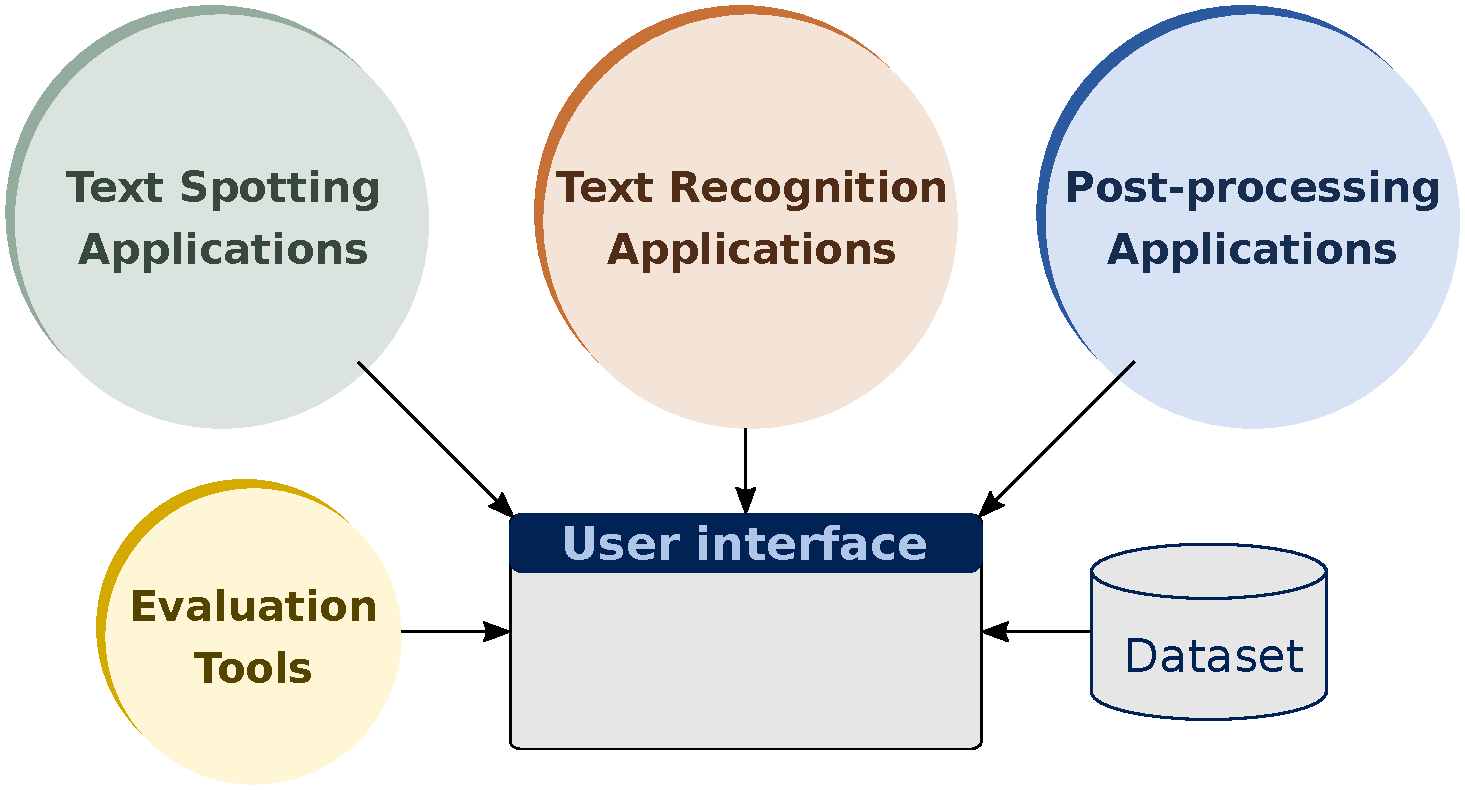
\includegraphics[width=0.6\textwidth]{E4/version-2/figs/prototype-overview-simple.pdf}
  \caption{Overview of the main components of the prototype. The text spotting applications refer to methods used for detecting candidate regions in a scene, while the post-processing applications are used to refine detection results. The text recognition applications provide the components responsible for recognizing texts found within detected regions.}
  \label{fig:prototype-overview-simple}
\end{figure}

\section{Architectural Overview}

The text recognition applications provide the components responsible for recognizing the text found within detected regions. The text localization module includes container applications that encapsulate the text localization methods used for comparison. The post-processing module comprises two containers: the post-processing method developed by the Samsung Research (SRBR) team, and an improved version. Similarly, the text recognition module provides three containers that encapsulate the three recognition methods: Tesseract, Long Short-Term Memory (LSTM), and Convolutional Recurrence Neural Network (CRNN) recognition methods. Table~\ref{tab:methods-available} summarizes the text detection and recognition methods handled in the tool.


\begin{table}[H]
  \centering
  \caption{Method for text detection and recognition available in the evaluation tool. For more detail refer to \cite{joselito}}
  \label{tab:methods-available}
  \begin{tabular}{lp{4.3cm}|p{4.3cm}}
    \hline
    \topline
    \headcol
    \textbf{Type}  & \textbf{Methods for Text Detection}    & \textbf{Methods for Text Recognition} \\ \midline
    & - SnooperText               	& - Tesseract v.3             \\
    & - Canny Text Detection          & \\
    & - MSER-SWT Text Detection         &  - Tesseract with Post-processing \\
   % & - Multi-Lingual Text Detection      & - Tesseract with Improved Post-processing \\
    & - FASText                 &                    \\
    
    \ml{-6}{*}{Non-Deep Methods}
    & - Scene Text Recognition &                    \\ \hline \hline
    & - SSTD                    & - LSTM (Tesseract v.4)         \\
    & - TextBoxes                 & - CRNN                 \\
    & - TextBoxes++                &                    \\
    & - SSD-MobilenetV2              &                    \\
    & - YOLOv3                   &                    \\
    
    \ml{-6}{*}{Deep Learning-Based 
      Methods}    & - SqueezeDet                 &                    \\
    \bottomlinec
  \end{tabular}
\end{table}

%\todo[inline]{Provide a description of said methods. Ask @Allan what is MSER-SWT and "Scene text recognition"
%R.: These are two non-deep methods for text localization that we exploit in the Deliverable E3. @Decker: You can found a description for these methods in the documents that I sent to you yesterday.}

\section{Implemented non-deep methods}

%\todo[inline]{Trocar tudo por uma versao da tabela do E1 e citar o joselito}
This section describes the non-deep methods implemented on the comparative tool. The deep-learning-based methods where already described in Section~\ref{sec:protocols}. Table~\ref{tab:non-deep-methods} presents the non-deep-learning methods considered in the tool. As we can observe, used methods include both region- and component-based approaches. Most of the methods rely on the use of classification systems that exploit shape and/or texture features in the identification of text regions.

\newpage

%\begin{landscape} % for rotate the page
  
  \begin{footnotesize}
    \begin{longtable}{p{.20\textwidth}|p{.20\textwidth}|p{.20\textwidth}|p{.20\textwidth}}
      \caption{Overview upon non-deep-based methods implemented on the comparative tool. For more details please refer to \cite{joselito}.}
      \label{tab:non-deep-methods}
      \endfirsthead
      \endhead
      \topline
      \headcol
       \bf Reference      
      & \bf Type 
      & \bf Features        
      & \bf Classifiers \\
       \midline
  
  
  Snooper text~\cite{Minetto2014CVIU}   
      & Region-based
      & Character filtering: Fourier descriptor, Pseudo-Zernike moments, and Polar descriptor. \newline
      Classification of text and non-text regions: T-HOG~\cite{Minetto2013PR}  
      & Character filtering: ensemble of SVM classifiers. \newline
      Classification of text and non-text regions: SVM \\\hline
  
    FASText~\cite{Buta2015} 
 
      & Component-based
      & Stroke-specific keypoint features
      & Adaboost classifier\\ \hline


  Canny~\cite{Cho2016CVPR} 

      & Component-based
      & Mean local binary pattern (MLBP) 
      & Two-round text classification with AdaBoost and multiple cascades
       \\ \hline
  
  MSER-SWT~\cite{Epshtein2010CVPR} 

      & Region-based and \newline Component-based
      & Stroke Width Transform 
      & Rules and thresholds based on the variance of the stroke
       \\ \hline
       
  Scene Text Recognition~\cite{Neumann2012CVPR} 

      & Component-based
      & Incrementally Computable Descriptors 
      & AdaBoost and SVM
       \\ \hline
      \bottomlinec

      %  \end{tabular}
      %\end{table}
    % \label{tab:non-deep}
    \end{longtable}
  \end{footnotesize}

\subsection{Recognition methods}
Three main recognition methods were implemented in the comparative tool: Tesseract, an LSTM-based approach and a CRNN-based approach. Tesseract~\cite{Smith2007ICDAR} is an open-source OCR engine proposed to recognize words from gray or RGB images, which can be understood as a five-stage pipeline. CRNN combines two types of neural networks, DCNN and RNN, to build an end-to-end system for sequence recognition, and T-LSTM is a Long Short-Term Memory (LSTM) network designed to recognize text lines. The LSTM is a special kind of Recurrent Neural Network (RNN) with the ability of learning long-term dependencies. The use of text recognition approaches is out of the scope of this dissertation. Readers may refer to~\cite{joselito} for a detailed description of such methods. 

\section{Implementation Overview}

The prototype developed in this chapter contains several applications with different software dependencies, including libraries, programming tools, and the base operating system. The integration of all these pieces of software into a single prototype is very challenging and we opted to package all applications that compose the prototype using the Docker\footnote{\url{https://www.docker.com/} (As of Jan 2020).} technology. Docker is an open source platform for operating-system-level virtualization. Docker provides a standardized unit software for packaging the source code and all its dependencies, including system tools, system libraries, and settings.

In this tool, we implement \textit{Dockerfiles}\footnote{Docker building configuration files.} that automatically package the source code, install its dependencies, install and compile source codes, and finally builds a docker image able to run the application as a command line, in a proper software platform. Figure~\ref{fig:overview-prototype} illustrates an overview of the architecture of the prototype. We built two base docker images, which contain some common libraries required for running non-deep- and deep-learning-based methods. These base docker images are used to build the docker images for the applications.
%\todo[inline]{padronizar ao longo da dissertação o uso de Figure and Fig.}
%
\begin{figure}[h!]
  \centering
  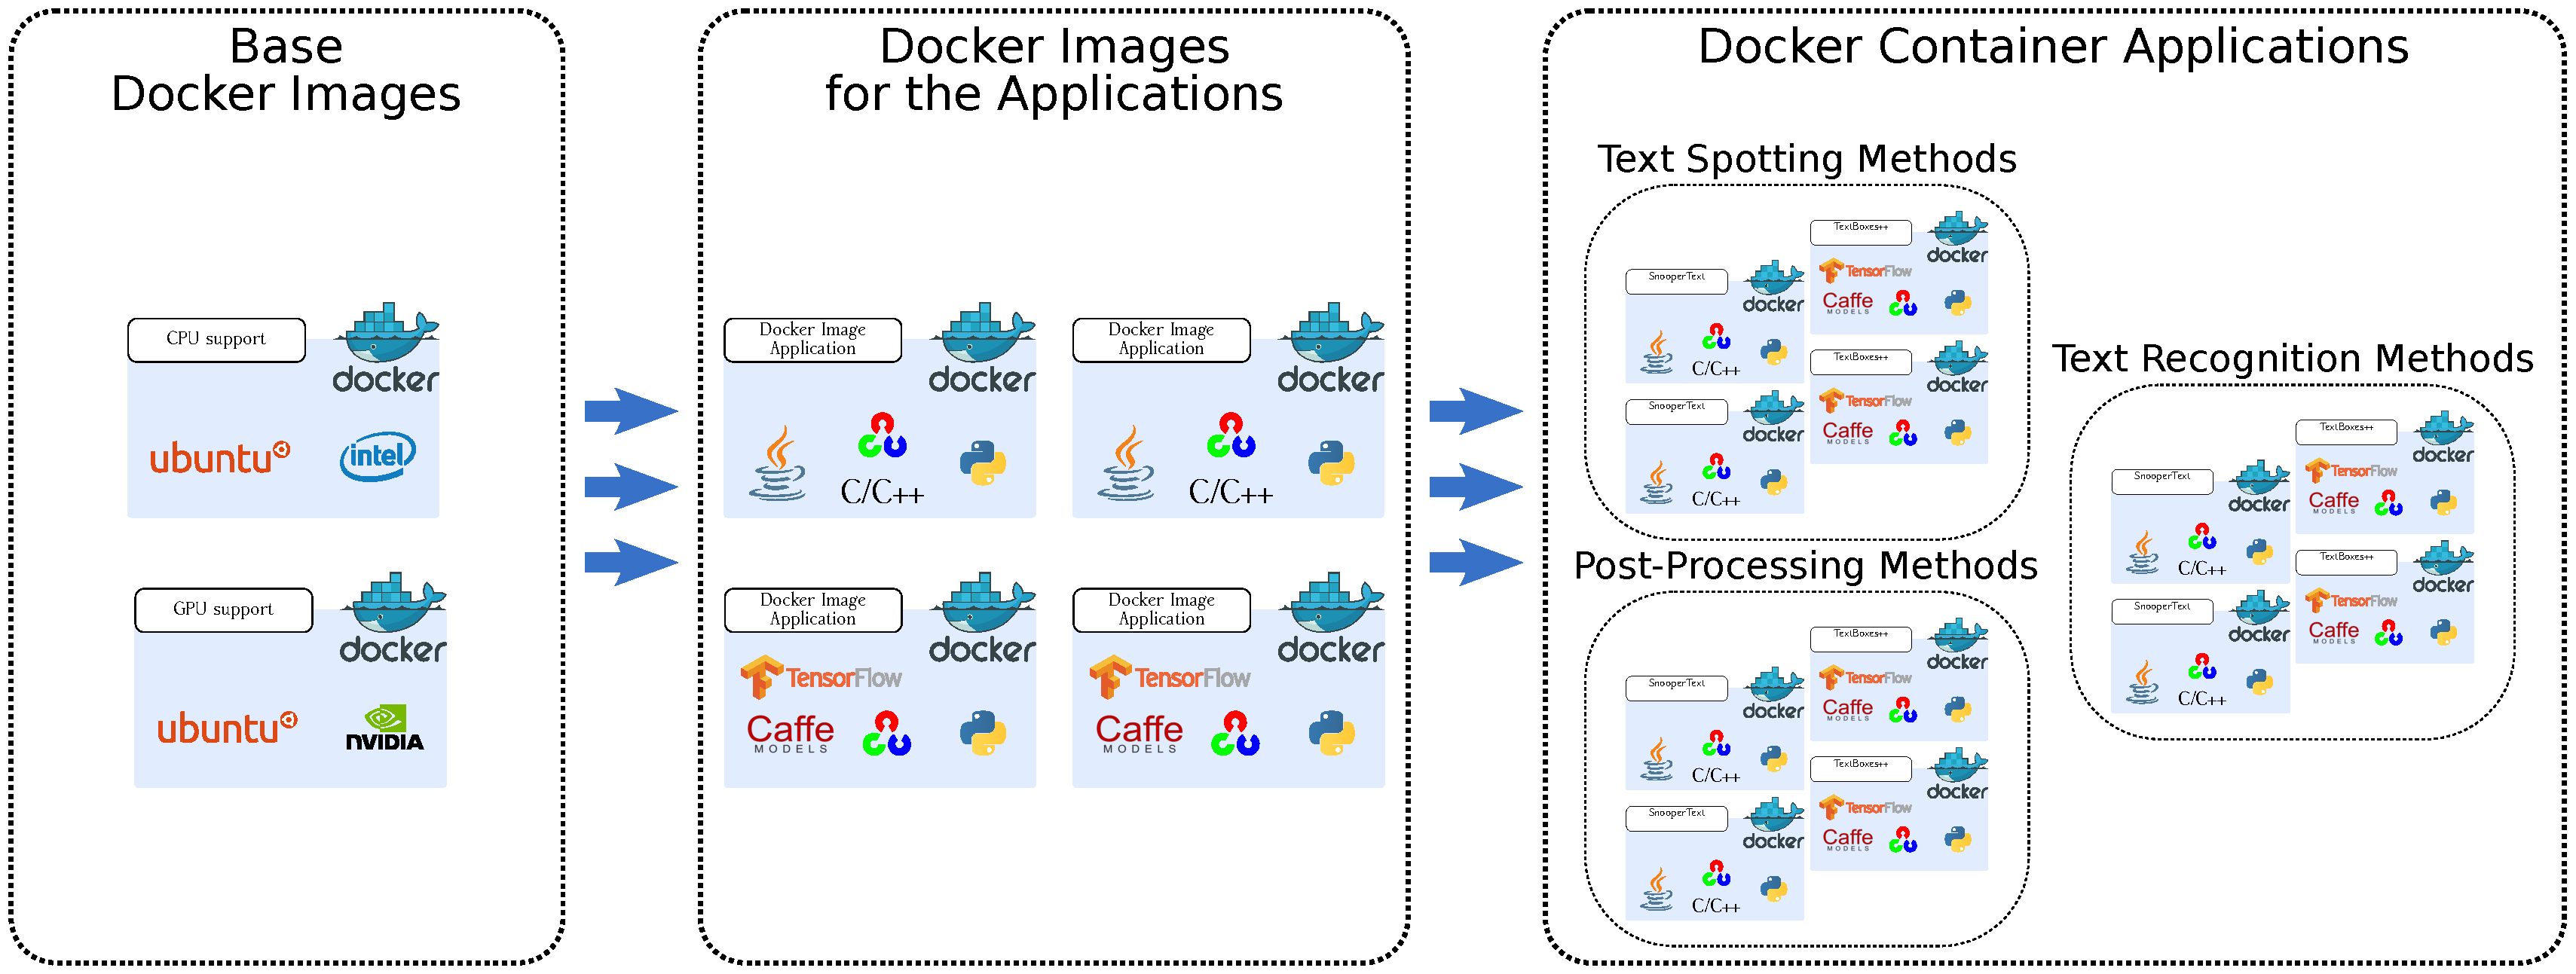
\includegraphics[width=0.98\textwidth]{E4/version-2/figs/prototype-overview.pdf}
  \caption{Architectural overview of the prototype.}
  \label{fig:overview-prototype}
\end{figure}

An overview regarding the use of the proposed tool in the context of the evaluation of text detection methods can be found in Appendix~\ref{app:code}.

%\todo[inline]{Incluir no apendice um exemplo de uso do megazord}


%SnooperText is a text detection approach introduced in~\cite{snooper}. This detector is composed of four main steps: image segmentation, character filtering, character grouping, and text region filtering. Initially, it locates candidate characters on images by means of a segmentation and a character/non-character binary classification system. The segmentation approach takes advantages of morphological operations for local contrast enhancement and thresholding. The classification system relies on shape descriptors (e.g., Fourier descriptors, Pseudo-Zernike moments, and Polar descriptor) and an ensemble of SVM classifiers. The candidate characters, represented by their bounding boxes, are then grouped according to geometric criteria. The resulting groups, i.e., candidate text regions, are validated by means of another texture-based classification system, which exploits a multi-cell histogram of oriented gradients (named T-HOG)~\cite{thog}, and another SVM~\cite{svm} classifier. All those steps are performed in multi-scale manner to address issues related to different character sizes and to avoid non-relevant texture details found within character regions.

%\subsection{Canny Text Detection}
%In this work, the authors present a novel scene text detection algorithm, Canny text detector~\cite{cannyTD}, which takes advantage of similarity between image. The proposed method can be summarized in five steps. In the first step, character candidates are extracted using extremal regions (ERs) method. YCrCb space color was used separately to extract ERs, as well their inverted channels. In the second step, a non-maximum suppression process is applied to reduce all repeating components produced by ER. In the third step, a double threshold classification is performed to classify surviving character candidates into three classes: strong text, weak text and non-text. Each character candidate is evaluated using an Adaboost classifier with multiple cascades. Two blocks of cascade classifiers are used, each with a threshold value of 99.0\% and 90.0\%. Mean Local binary pattern (MLBP) is used as the descriptor, which is robust to illumination and rotation variations. In the double threshold classification, all candidates go through the first cascade block and are classified as strong text or non-strong text. Non-strong text candidates go through the second cascade block, which in turn classifies them as weak or non-text. In the fourth step, a text-tracking-based on hysteresis is applied, strong text are included in the final result because they are classified with high confidence. Weak text can be either classified as true text or not-text, so they are included as high confidence if they have similar properties to strong text candidates. In the fifth step, a text grouping process is applied, two candidates are compared based on spatial location, size, color, and aspect ratio using the same threshold values (99.0\% and 90.0\%). If they satisfy the properties, then they are grouped into a same word.

%\subsection{FASText}

%Busta et al.~\cite{fastext} introduced FASText. FASText is a stroke detector based on an efficient pixel intensity comparison to surrounding pixels. FASText is based on four main steps. In the first step, to detect stroke-specific keypoints efficiently, two keypoints classes were introduced: the stroke Ending Keypoint (SEK) fires on a stroke ending, whilst the Stroke Bend Keypoint (SBK) fires on a curved segment of a stroke. Four parameters are used to detect keypoints: circle size, margin, scaling factor, and the maximum number of keypoints. In a second step, a threshold value is found directly from FASText keypoint to segment individual characters from the background. In the third step, to reduce false detection, an efficient classification component is employed. Inspired by the MSER segmentation classifier~\cite{Neumann2015ICDAR}, an AdaBoost is used as a classifier. Compactness, convex hull are ratio, holes area ratio and the character Stroke Area (CSA) are used as features to classify FASText regions as a character or background clutter. CSA feature is based on the observation that the area of an ideal stroke is the product of the stroke width and the length of the stroke.
%In the fourth step, an unordered set of FASText regions classified as text fragment (characters) are clustered together to form lines of text. A standard (approximate) nearest-neighbor algorithm is used for this process.

%\subsection{Scene Text Detection}
%Yi et al.~\cite{Yi2014TIP} address the problem of performing scene text detection and recognition in mobile devices. Character detection is based on the combination of bags of visual words and Gaussian mixture models computed based on HOG features extracted from points defined by four different detectors. Later, stroke configuration maps, defined in terms of character boundary and skeleton, are used to model the character structure for different classes. Target applications refer to text understanding and retrieval.

%\subsection{Multi-lingual}
%33333This proposal~\cite{multilingual} presents a technique for multi-lingual video text recognition which involves script identification in the first stage followed by word and character recognition and finally the results are refined using a post-processing technique. Considering the inherent problems in videos, a Spatial Pyramid Matching (SPM) based technique, using patch-based SIFT descriptors and SVM classifier, is employed for script identification. In the next stage, a Hidden Markov Model (HMM) based approach is used for word and character recognition, which utilizes the context information. Finally, a lexicon-based post-processing technique is applied to verify and refine the word recognition results.

%\subsection{Tesseract}

%Tesseract~\cite{Smith2007ICDAR} is an open-source OCR engine proposed to recognize words from gray or RGB images, which can be understood as a five-stage pipeline. Firstly, the input image (text region) is converted to a binary image using an adaptive threshold. This image is segmented via a connected component analysis method for further inspection of the nesting of outline and also to deal with write-on-black text regions. At this point, the Tesseract provides a set of blobs with nested outlines gather together in order to have an organization of text line regions. The next stage of the method consists of finding text lines by filtering out regions with a height smaller than a threshold $\delta$, which is defined as the fraction of the median height of the text size in that region. Later, the Least Median of Square method~\cite{Rousseeuw1987Wiley} is applied in order to find the baselines and a fixed and non-fixed pitch detection is applied to split words into characters. Finally, a two-step classification process is used to recognize characters, considering a set of topological features~\cite{Shillman1974MIT,Blesser1976PR}, such as y-position relative to baseline, contour length, second x-moment, and second y-moment.